Deep learning models require tremendous amounts of data, to ensure the model works well the data must also possess sufficient characteristics to approximate the sample population from which it was extracted. To satisfy this requirement we examine the data in attempt to remove outliers and determine whether the data is sufficient for classification. Moreover, certain tumors may be heterogeneous \cite{friedmann2014glioblastoma}, which may be problematic for a classifier as heterogeneous samples lack in shared characteristics. In this chapter the data available to the project is examined in greater detail; details for how the Raman spectra were prepared is given to document the preprocessing of spectra for future use. First we describe the mathematical representation of the samples. Since the number of samples is too small to use in a deep learning model, we explain how each sample may be separated into individual spectra; this separation yields a drastic increase in the number of available training examples. We then explain how to balance the data; an unbalanced dataset would likely introduce bias in the deep learning model, rendering its desired predictive capabilities uncertain. We achieve this by duplicating underrepresented samples-classes in the dataset. Furthermore, this balancing is performed to maintain majority and minority classes, thus retaining some distributional information from the original dataset. The quintessential purpose of this chapter is to analyze the data using k-means clustering and hierarchical clustering for detecting non-tumor spectra or otherwise erroneous spectra. These methods are tested in contrast to other outlier detection techniques such as the standard deviation test and the interquartile range method. Adrian's criterion is presented and compared to the the spectral images extracted from the samples.
Another point of interest in this project is the identification of representative frequencies within the spectra. Each spectra belongs to a tumor which can be categorized by six different classes. The hypothesis states certain frequencies should be sufficient in determining which class the tumor belongs to. For this feature selection is used, representing each frequency within the spectra as distinct features. This task is simplified by the new representation of the data separated into lists of spectra rather than a collection of spectra represented by the tumor. However in order to extract such features the data must be devoid of outliers. Should outliers exist within the dataset, the features given by the methods used will be influenced and may yield conflicting results with the ground truth. To prepare for this the data is plotted for visual inspection using various methods to be discussed in the following section on feature selection. It is confirmed by the provider that the majority of samples include faulty spectra e.g. spectra of blood drops on the sample or plastic which may be reflected form underneath thin tissue. Furthermore some tissue may be necrotic which will affect the spectral signal. Using the extracted features a model can potentially form around the data faster which can be essential as deep learning training require significant computing resources. The features are extracted before and after the removal of problematic spectra for comparison.


\section{Data Representation}
The data consists of the Raman-spectra extracted from the tissue of glioma tumors from 45 patients. Multiple samples of tissue were extracted from the same patient in some cases, yielding several samples for the respective patient. To maintain separation among the patients, the samples are sorted by their respective patient of origin. This is necessary, since there is uncertainty regarding the homogeneity among patient samples. The data will be separated into three separate datasets. These sets are called training set, validation set and testing set. All datasets will consist of unique patients to avoid scenarios in which the model overfits to a patients tumor sample and as a result of heterogeneity. This structure also allows for easier handling of the number of patients in the sample-classes, allowing for analysis on each class exclusively. 

There is also large variation with regard to the sample shape within the data. Each sample is a 3-dimensional array of shape $(w, h, 1738)$ where $w$ and $h$ are the width and height of the sample, respectively. This formalization is necessary, as width and height have non-zero variance among different samples. The shape is a result of how the tissue was scanned. In each case the tissue was placed inside the instrument and scanned successively from side to side. This makes it possible to display each sample as an image, by substituting the third dimension (denoted above by $1738$) a color value denoted by which class the spectra belongs to. The number $1738$ is constant through all samples and represents the length of a modified Raman-spectra which is performed by the provider, each element a unique frequency. Furthermore each element inside these arrays is a real number without clear bounds. The largest absolute element found within the complete dataset is $79427.0625$, some values are negative which is confirmed by the providers to have significance for the projects purpose. The project aims to predict which subdivision the spectra belong to by feeding in one of these samples, i.e., one vector of shape $(1, 1738)$. This strategy is inspired by Liu et al.\cite{liu2017deep}, who managed to get satisfactory performance by training a model on raw spectra. This representation is of great interest, since the value of each spectrum is independent from the surrounding spectra. Separation at this level yields a dataset with more than $300,000$ datapoints, which better suits deep learning tasks.

 
To prepare for the project each samples spectra is collected and plotted in one single plot to compare spectral information from the sample itself. An example of such plots can be seen in Appendix \ref{appendix:spectraplot}. Patient HF-1887 is removed from the project completely due to the skewed baseline in the spectra.


\section{Data preparation}
In this section we explain our qualitative analysis on the data, done to determine the plausibility of our model. Each sample is categorized according to their subdivision; there are six distinct subdivisions as defined by Ceccarelli et al. \cite{cellsubsets}, denoted LGm1 - 6. As an initial step each samples spectra is analyzed by visual inspection. The spectra are plotted on a two dimensional surface as lines, each line a unique spectrum. Through this analysis one sample is discarded due to the tilted baseline of the spectra, none of the other samples share this problem. A sample which shares a general shape with the other samples is shown in contrast to the sample selected for removal in \ref{appendix:spectraplot}. Another sample shows a concerning number of spikes in contrast to the other samples. The number of spectra is also considerably larger compared to the others, which is limiting for some of the methods selected for the analysis. For this reason the sample is also discarded.

\subsection{Organization and Balance}
The model will as a consequence of it's learning-algorithm become biased towards certain predictions. This because as the model encounters frequent examples of a certain class, the connections which produce such predictions will strengthen. Over exposure to examples of a certain class will force the model to associate features with that class, redirecting focus from classes for which that feature could be significant. The initial data suffers heavily from this problem, a is shown in Table \ref{table:1}.

\newpage

\begin{table}[h!]
\centering
 \begin{tabular}{||c c c c c c c||} 
 \hline
 Class & LGm1 & LGm2 & LGm3 & LGm4 & LGm5 & LGm6 \\ [0.5ex] 
 \hline\hline
 \# of samples & 5& 11 & 4 & 10 & 11 & 4 \\ 
 \hline
 \# of spectra & 37319 & 71846 & 31931 & 50660 & 62256 & 20176 \\
 \hline
 percentage & 14\%& 26\% & 12\% & 18\% & 23\% & 7\% \\
 \hline

\end{tabular}
\caption{Table showing the distribution of data in the initial dataset after removing the problematic samples. The number of samples are displayed on the first row, the number of spectra in each class is shown on the second row. The percentage of the entire dataset is shown on the third row. The majority class is LGm 2 and minority is LGm 6.  Classes LGm 1, 3 and 6 must be expanded to balance the data.}
\label{table:1}
\end{table}

Table \ref{table:1} shows the per class separation in the data, the header row shows the labels of each class. The first row shows the number of samples belonging to each class, these are the tumors which will be analyzed. The second row displays the total number of spectra across each class; these must be considered for balancing. Note the equal amount of samples in LGm3 and LGm6, but the difference in number of spectra within them. This is due to the varying size of all samples drawn from the tumors. Some samples share the same size, however the important fact is that the samples lack a uniform shape, which must be considered during the analysis. The last row shows the percentage each class makes of the entire dataset. Initially LGm2 is the majority class while LGm6 is the minority, consisting of only $7$\% of the entire dataset.

Before the data is balanced, the testing data is selected and separated from the rest manually. This is done by separating at least one patient and all their samples from the rest of the data. This way it will be possible to test if the model is develops bias towards the patients in training and if the patient samples are heterogeneous with respect to the other samples of the same class. The test-samples are chosen manually, samples are chosen with the criterion that approximately $30\%$ of each class is represented in the test set. Balancing the classes which contain less elements by a factor larger than or equal to two compared to the majority class (LGm2) is done by repeating the spectrum in each sample by that factor. Following this method the majority class will stay the majority which can be crucial provided the sample pattern is similar to the set of all other unseen samples. The resulting dataset is gained by doubling the samples in LGm1, tripling the samples in LGm3 and quadroupling the samples in LGm6. The distributions of the training dataset is shown in Table \ref{table:2}.
\\
\\
\begin{table}[htb]
\centering
 \begin{tabular}{||c c c c c c c||} 
 \hline
 Class & LGm1 & LGm2 & LGm3 & LGm4 & LGm5 & LGm6 \\ [0.5ex] 
 \hline\hline
 \# train & 21289	& 51698	& 20635	& 34276	& 37492	& 12976 \\
 \hline 
 \# test & 14945 & 20140 & 11296 & 16384 & 24764 & 7200 \\
 \hline

\end{tabular}[htb]
\caption{Distribution of the training data and the testing data}
\label{table:2}
\end{table}

Table \ref{table:3} shows the distribution of the training data and testing-data. The training data is then balanced exclusively. This is not required in the testing data, since it will have no effect on how the model is developed through training. The training data is balanced by replicating each spectra in every patient of the classes which are under-represented. The resulting training-set is gained by doubling the spectra in LGm 1 and LGM 3 and  the spectra in LGm 6. The final distribution of the training data following this procedure is shown in table \ref{table:3}

\begin{table}[htb]
\centering
 \begin{tabular}{||c c c c c c c||} 
 \hline
 Class & LGm1 & LGm2 & LGm3 & LGm4 & LGm5 & LGm6 \\ [0.5ex] 
 \hline\hline
 \# train & 42578 & 51698 & 41270 & 34276 & 37492 & 38928 \\
 \hline 

\end{tabular}
\caption{Distribution of the testing data following balancing}
\label{table:3}
\end{table}

\section{Analysis}

Following the balancing, the first step in the analysis is to find the frequencies which best describe the data with respect to the methylation-types. Each number in the spectra is a frequency at which the scattered light is gathered. This light is expected to be sufficient for predicting the methylation-type of the tumor-tissue. It is speculated that to sufficiently categorize the spectra into the methylation-types only certain frequencies are required. For this reason the best features are extracted with SelectKBestfeatures \cite{scikit} which is given the f-classif method for ranking the features which yields features deemed significant by ANOVA. The 70 best features were extracted from the training-data in which there are spectra which originate from non-tumor tissue. The features are displayed in Appendix \ref{appendix:features0}. Before the features are extracted, each spectra is standardized using z-score standardization, to give each spectrum a mean of zero and a standard deviation of one. This is done for ease of comparison among the spectra. The extracted features show that regions of interest do exist on the spectra. This can be seen by the integers which have a difference of one, suggesting that the region of interest exist somewhere in specific parts of the spectra. It is worth noting here that the features selected might be correct provided the amount of non-tumor spectra is sufficiently small to be ignored by the feature selection method. Due to this uncertainty, the data will be separated from the outliers and feature selection will be performed a second time.

All data is subject to this analysis as all samples must be cleaned of outliers before the model can be trained. In the methods where statistical constants must be calculated, the training data is used, this avoids bias towards the other datasets whose primary purpose is to evaluate the model. The goal of the analysis is to find a uniform criterion which each spectrum must fulfill to be considered \textit{clean}. Spectra which fail to satisfy this criterion will be discarded form the project entirely. In this section the methods of analysis used are described and their results examined, the section begins by examining the standard deviation test and interquartile range method, these are deterministic methods that rely solely on the values found within the data. K-means clustering and Hierarchical clustering are then performed on the data in attempt to capture potentially complex patterns within the data. The section ends by presenting Adrians criterion, which is a confirmed criterion all spectra must satisfy to be considered legitimate spectra (also refered to ass \textit{"clean"}).

\subsection{The standard deviation test}

The standard deviation test is a test by which the data is centered around the mean and given a standard deviation of one. With this setup, outliers are defined as points which are separated from the mean by three standard deviations or more. We measure the mean and standard deviation on each frequency from the unbalanced training-set; the values are then used to standardize the spectra belonging to each tumor. A spectrum is deemed to be an outlier if the number of frequencies in that spectrum exceed an arbitrary value. We approximated the value by performing the test once while monitoring the average number of frequencies which lie three or more standard deviations from the mean. In any given sample, each spectrum includes on average $111$ frequencies which fail the test. We specify that a spectrum whose number of frequencies which fail the test is a spectrum possessing more than $111$ outlier-freuencies, is deemed an outlier. 

Using this test, many small areas are detected in each sample, it suggests there is something present in those places, but they do not possess a clear shape by which we can decide whether to discard them or not. An example of such a sample is shown in Figure \ref{fig:stdHF448}.

\begin{figure}[H]

    \centering
{\includegraphics[width=4cm]{images/STDtest/LGm-1/HF-448_V5B_1.h5_3.png} }
\caption{Sample HF-448 from LGm1, The test fails to detect outliers and falsely labels healthy tissue as outliers.\label{fig:stdHF448}}%

\end{figure}

Roughly $50\%$ of the samples in the entire dataset yield similar results from this analysis. The method would as a result discard too much from most samples, depraving the dataset of a great number of tumor spectra. Some areas are formed around the individual spots, suggesting the presence of an unknown material, but the sporadic points in the surrounding area make it unclear where that material begins and ends. Furthermore, we must develop a criterion for which points to discard. Such a criterion would need to distinguish between sporadic points which are miss-classified and areas of real outliers.

However, within some samples there are clear areas of outliers, but those areas are not sufficiently defined. One sample with this result is shown in Figure \ref{fig:stdHF868}.

\begin{figure}[H]
	\centering
{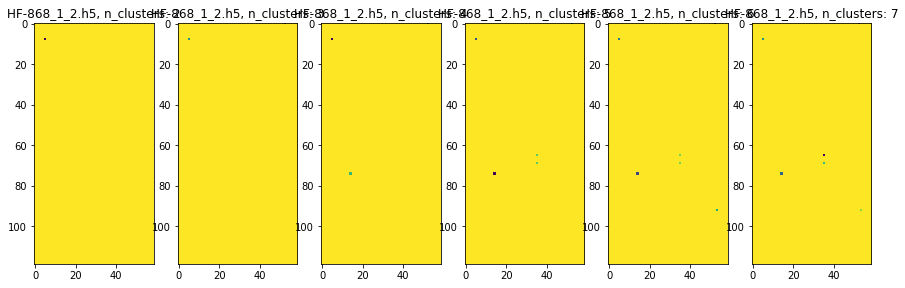
\includegraphics[width=3cm]{images/STDtest/LGm-1/HF-868_1_2.h5_0.png} }
\caption{Sample HF-868 from LGm1, Several of the captured areas are confirmed to be outliers, but they fail to adequately capture all erroneous spots.
\label{fig:stdHF868}}

\end{figure}

Sample HF-868 is less sporadic compared to HF-448, the outliers are instead formed around common points of interest which strongly suggests non-tumor spectra are present in that area. The lack of definition in each area however, is not sufficient. The outliers must form concrete shapes with clear definition. The sample suggests outliers in the different areas, but all points are not present to make the shapes apparent. 
The sporadic results show that this method is insufficient to detect the majority of outliers in all samples. It must be noted that despite this underwhelming result, some outliers are detected, suggesting further changes to the method could yield better results, though greedy application is not going to work for all samples. Throughout all the six LGm-classes, the method yields the best results for LGm6 where it shares many patterns with the patterns produced by \textbf{ADRIANS CRITERION} (covered in a later section). Another example of the methods promise is in sample HF-2852 of LGm3 shown in Figure \ref{fig:stdHF2852}.

\begin{figure}[H]
	\centering
{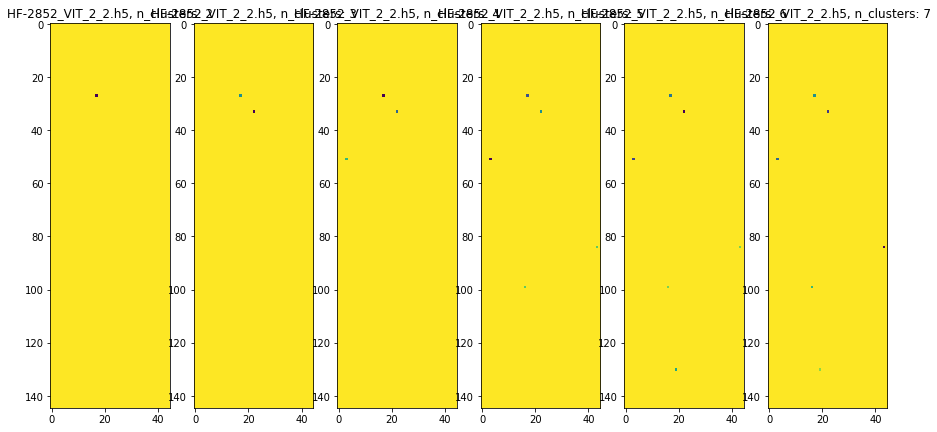
\includegraphics[width=3cm]{images/STDtest/LGm-3/HF-2852_VIT_2_2.h5_6.png} }
\caption{Sample HF-2852 from LGm3. A large area in the upper part is captured, confirmed to be nectrotic tissue.
\label{fig:stdHF2852}}

\end{figure}

Sample HF-2852 has a large area in the upper part which consists of necrotic tissue. The spectra of that tissue differs from other spectra sufficiently well, allowing the method to distinguish between tumor and non-tumor with considerable accuracy. This is due to the amount of otherwise healthy tissue present in the sample. The methods inability to capture all outliers is also present despite this, as it allows several smaller spots in the area of the necrotic tissue to be classified as healthy tumor tissue. These results suggests that the method is best used in detecting necrotic tissue, but not in context of detecting other kinds of outliers.

\subsection{The Interquartile range method}

Similar to the standard deviation test, the interquartile range method is a purely statistical analysis method which detects outliers in terms of which percentile the spectra belong to. The 25th and 75th percentiles are calculated on each frequency for the entire training set. Like the previous test, this method yields a varying amount of outliers for each sample. We instead define the allowed number of outlier frequencies within one spectra to be equal to the average number of outlier frequencies within the analyzed sample. Many regions are better represented by the interquartile range, showing well defined areas where non-tumor tissue is clearly present. The amount of individual spots are less frequent which shows promise in the method, as e.g. blood is expected to cover a larger area if present. The improvement from the standard deviation test is seen in Figure \ref{fig:iqrHF448}.

\begin{figure}[H]

    \centering
    \subfloat[\centering The result of the interquartile range for HF-448, Several well defined areas are separated form the majority of spectra]{{\includegraphics[width=4cm]{images/IQR/LGm-1/HF-448_V5B_1.h5_3.png} }}
    \qquad
    \subfloat[\centering The standard deviation test for sample HF-448]{{\includegraphics[width=4cm]{images/STDtest/LGm-1/HF-448_V5B_1.h5_3.png} }}%
    \caption{A comparison between the interquartile range and the standard deviation test for sample HF-448.
\label{fig:iqrHF448}}%
\end{figure}

The standard deviation test failed to separate outliers adequately in sample HF-448 while the interquartile range is better suited to detect the outliers in this sample. The upper part of the sample has a well defined line where the sample is presumably cut, meaning the plastic underneath the tissue might be visible. We also note that many outliers detected by the interquartile range also appear to be captured by the standard deviation test. While the areas are hard to distinguish among all sporadic spots, the larger spots in Figure \ref{fig:iqrHF448} (a) seem to have some trace in Figure \ref{fig:iqrHF448} (b). This further shows the methods capability in contrast to the standard deviation test as the method seem to possess greater ability in defining the areas where outliers are present. There are still some spots appearing randomly around the sample surface which would ideally be ignored, but while we have some confirmation on where outliers are present in certain samples, we do not know exactly where the outliers are. The individual points being labeled as outliers suggests the method struggles with the same issue the standard deviation test suffers from. Though it appears to be less severe in all samples belonging to LGm1, there are still a considerable amount of spots through all samples within the class. Especially LGm4 have samples for which both methods perform considerably poorly, with a considerable amount of sporadic spots appearing in some samples under the interquartile range and a significant lack of spots under the standard deviation test. This issue is apparent in sample HF-2802 of LGm4, shown in Figure \ref{fig:HF2802comp}.

\begin{figure}[h]

    \centering
    \subfloat[\centering The result of the interquartile range for HF-2802, some larger areas are detected with sporadic spots around the entire spectra.]{{\includegraphics[width=4cm]{images/IQR/LGm-4/HF-2802_V3T_1.h5_11.png} }}
    \qquad
    \subfloat[\centering The result of the standard deviation test for HF-2802. Few outliers are detected]{{\includegraphics[width=4cm]{images/STDtest/LGm-4/HF-2802_V3T_1.h5_11.png} }}%
    \caption{A comparison between the interquartile range and the standard deviation test for sample HF-2802. In comparison, the interquartile range locates better defined areas than the standard deviation test, but many sporadic spots are present.
\label{fig:HF2802comp}}%
\end{figure}
 

In Figure \ref{fig:HF2802comp} the results of both methods are compared on sample HF-2802. Both methods yield poor separation between the outliers and tumor spectra. The interquartile range is capable of detecting a large mass of some material on the sample, however, many sporadic spots appear around it, the majority of these spots are tumor spectra which would be discarded by the method. In stark contrast the standard deviation test struggles to detect anything in the sample, only yielding small spots in the larger areas found with the interquartiale range method.
Fewer samples suffer from the stocastic results present in the standard deviation test, however all samples are not strictly improvements from the previous test. One such example is sample HF-1010 shown in Figure \ref{fig:HF1010comp}.

\begin{figure}[h]

    \centering
    \subfloat[\centering The result of the interquartile range for HF-1010, a considerable number of spectra are falsely labeled as outliers]{{\includegraphics[width=4cm]{images/IQR/LGm-2/HF-1010_V1T_1.h5_8.png} }}
    \qquad
    \subfloat[\centering The result of the standard deviation test for HF-1010. Few points are selected and the areas found correspond with known outlier positions]{{\includegraphics[width=4cm]{images/STDtest/LGm-2/HF-1010_V1T_1.h5_8.png} }}%
    \caption{A comparison between the interquartile range and the standard deviation test for sample HF-1010.
\label{fig:HF1010comp}}%
\end{figure}

The comparison in Figure \ref{fig:HF1010comp} show one of few samples where the method fails to sufficiently separate outliers from tumor spectra. Few samples follow the same conclusion, however, the results suggest the method is unsuitable for our purposes. 

\subsection{Hierarchical clustering}

The next method of analysis for outliers is hierarchical clustering, we choose to utilize agglomerative clustering as an arbitrary choice. Due to the algorithms demanding time complexity and memory constraints, we choose to analyze each sample separately to avoid these issues. This means there is little to gain in comparison among separate samples however the deterministic nature of the algorithm shows promise for rigorous results in the clusters. We compare the results of different distance metrics and choose to utilize Euclidean distance to measure distance among the clusters. This conclusion is due to the uncertainty in vector shape and angles on which Cosine similarity is dependent. The Manhattan distance would be a better choice compared to Cosine similarity, however, Euclidean distance magnifies long distances which should aid the algorithm in selecting clusters for agglomerative merging. Following choice of distance metric we examine the linkage criteria available. In each case, the algorithm is set to run multiple tests where it separates the data into different amounts of clusters. We choose to compute between $2$ and $7$ clusters.

Single linkage merges clusters by way of merging those which posses points with minimal distance. One flaw in this criterion is that clusters may easily be merged from one parent cluster until all points have been connected in a chain. The criterion yields clusters which appear as individual points in the spectra and fail to detect areas where known outliers are present in the samples, suggesting the aforementioned flaw is present in this methodology. This is especially apparent if we allow the method to use more than two clusters. All different cluster amounts fail to separate the outliers and instead separate a small number of points. Examples of these cluster results are displayed in \textbf{Appendix}.

Average linkage yield similar results as single linkage with the exception that some areas become apparent as we increase the number of clusters. Moreover, the criterion does not have a set number of clusters which is guaranteed to include all outliers. For certain samples the outliers are visible when forcing the algorithm to agglomerate to two clusters and others only show them once five or more clusters are allowed. It is possible to use the criterion for discarding the outliers if the majority cluster is preserved when computing 7 clusters while the rest of the spectra are discarded, but this would not remove all outliers and some problematic samples in LGm3 would have the majority of outliers preserved. 

Complete linkage merges the clusters which posses elements with the smallest possible maximal distance between them. This avoids the setback of single linkage as a majority cluster is harder to form early under the criterion. The method produces similar results as average linkage, few areas with outliers are detected when fewer clusters are permitted. However, some outliers are present when computing 2 or 3 clusters. Allowing 7 clusters to form allows the algorithm to capture many of the areas of interest, however, this captures too much in some samples. We recommend the majority cluster is maintained when allowing 4 clusters with the method. But this suffers from the same setback as our conclusion on average linkage.

Ward linkage merges clusters which posses minimal variance between their respective elements and as such works well with Euclidean distance. We do stress that the clusters are merged by measuring variance among cluster elements and there is no guarantee the outlier spectra should share in characteristics which would result in low inter-cluster variance. Despite this lack of guarantee the clusters form at the precise location of outliers. Allowing 7 clusters produce a near picture perfect image of the biological tissue from which the spectra were measured. These results show that the algorithm is capable of organizing the spectra according to their visual information which aid us in understanding shape and state of the samples. Some of the spectral images fromed by the clusters are shown in \textbf{Appendix}. The issue is finding a uniform criterion on which we can discard the outliers. Removing every cluster except for the majority cluster in the case where 7 clusters have been formed would remove legitimate spectra which are suitable for training a model. In fact, there is no optimal choice in this case, as certain samples have their outliers sufficiently captured in a setup allowing for 2 clusters. While others show their outliers in arbitrary numbers of clusters. Selecting too many clusters will result in some samples loosing legitimate spectra which is undesirable in context of maintaining a sizable dataset. By visual inspection, we deem the optimal choice to be 3 clusters since many outliers are present in this choice, though the problem is still present in this alternative. In particular, sample HF-2485 suffers from this problem, the cluster results are shown in Figure \ref{fig:hf_2485}.

\begin{figure}[h]

    \centering
{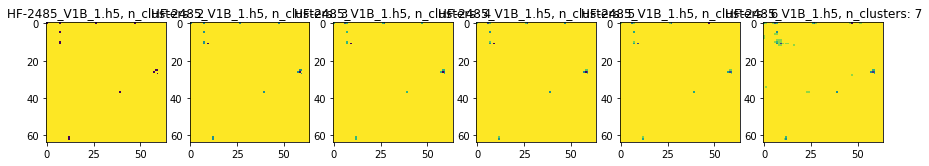
\includegraphics[width=15cm]{images/Ward_linkage/LGm-5/HF-2485_V1B_1.h5_9.png} }
\caption{Sample HF-2485 from LGm5, clustered by Hierarchical clustering using Ward linkage. From left to right, is shown the results of computing from 2 to 7 clusters respectively. The oultliers are present from image 4 and up.
\label{fig:hf_2485}}%
\end{figure}

 The model separates much of the healthy tissue in models computing 3 clusters or fewer. In the model computing 4 clusters, the utliers are visible as dark spots which perfectly correlates with the image of the tissue. The surface of the tissue is also well represented in the model computing 7 clusters.

\subsection{K-means clustering}

We continue this analysis by performing K-means clustering in attempt to separate the outliers. We flatten the training data and reorganize it in random order to avoid bias towards recurrent LGm-classes in the dataset. The examples are then used to fit 5 K-means models to compute 2 to 7 clusters respectively. This method has the advantage of being trained on the entire training set whereas Hierarchical clustering possesses too great a time and space complexity which makes similar experiments impossible with our current hardware. Under this structure we may now compare the results between sample predictions. We observe that the stochastic nature of the algorithm produce results of varying quality. In contrast to Hierarchical clustering, K-means do not produce clusters as subdivisions of previously seen clusters. This is due to the algorithm being computed several times with different initialization settings. The final result which the algorithm yields is the cluster state possessing minimal inertia compared to the other computations. Compared to all other methods of analysis, this method is able to capture small segments of the upper part of the sample HF-1293, shown in Appendix \ref{appendix:spectralimages}. While the comparison among the different models created loses some credibility in this setting, the comparison between the model results among the different samples are promising. We find that the model in which two clusters are computed, the samples are divided in ways which corresponds with Adrians criterion (explained in the next section) whereas samples where minimal amounts outliers are present the clusters seem to form around healthy tissue, which in turn create an image resembling the surface of the sample-tissue. In certain cases the clusters fail to capture known outliers but other models allowing for more clusters capture them sufficiently well. One example of this is sample HF-868 where the two cluster model fails to detect the relevant outliers but the model computing 3 clusters capture the outliers in near perfect resemblance to Adrians criterion. The other models however then loose some of the outliers around the shapes present while still capturing the center of the shapes. The likeness to Adrians criterion returns in the model computing 6 clusters but this is again lost in the model computing 7 clusters. And like Ward linkage for Hierarchical clustering, there are some samples where the majority cluster is hard to evaluate, one such sample is HF-2544 which shifts the majority cluster between the model computing 2 clusters and the rest of the models. Due to the variety among the different models finding a uniform criterion for detecting outliers is problematic. Many samples are such that the models steadily increase the number of outliers clustered, but this relationship is not constant through all samples, making it insufficient for use in the hypothetical criterion. The shifting of majority cluster in the aforementioned sample further complicates matters, since the majority cluster may not be capturing healthy tissue in some samples. For this reason we deem the method insufficient for separating outliers though we add we note its promise in capturing information about the tissues visual aspects, which makes the method comparable to Ward linkage for Hierarchical clustering. 

\subsection{Adrians criterion}

Adrians criterion is a criterion specified by Adrian Lita for separating outlier spectra from the rest. The criterion states: should any value of frequencies between $1463$ and $1473$ of any spectrum be below $5000$, then that spectrum is defined to be and outlier. Given that this criterion is defined by the provider, and the lack of consistency in the other methods explained in this section, we choose to discard outliers found by Adrians criterion despite the criterion missing certain areas such as the upper part of sample HF-1293 which does not satisfy the criterion, but is also confirmed to be plastic. Our hope is that the model will be able to ignore these and other potential outliers which escape Adrians criterion.
\\

Concluding this section we also perform clustering with the selected features gained from the beginning of this section \textbf{Reffer to appendix for this!}. Limiting the spectra to the features which best separate them into the 6 LGm-classes has advantage for this algorithm, many areas of outliers become easily spotted by allowing 2 clusters in many cases. Complete linkage gains the biggest advantage out of this method. None of the above mentioned configurations manage to capture the upper part of HF-1293, however, when the data is limited to the features selected, the area becomes visible to some extent. This suggests there are frequencies in the spectra which complicate the separation of outliers. While we see that the method clearly works in many cases, using all features proves to be troublesome for the majority of linkage criteria. Furthermore, the features are computed by means of separating the spectra into the 6 LGm-classes, they are not computed due to their efficiency for detecting legitimate spectra and outlier spectra. Following the removal of outlier spectra we decide to label each spectrum by a binary value, a spectrum is assigned true if it is legitimate and false if it is labeled an outlier by Adrians criterion. We then run feature selection once more, extracting the features which bets separate legitimate spectra from outliers. The features are displayed in Appendix \textbf{appendix:Features}.